\section{Application et limites}
\begin{frame}{Application sur une image de zoo}
\begin{figure}
\begin{center}
\begin{tabular}{ccc}
\subfloat[Image réduite]{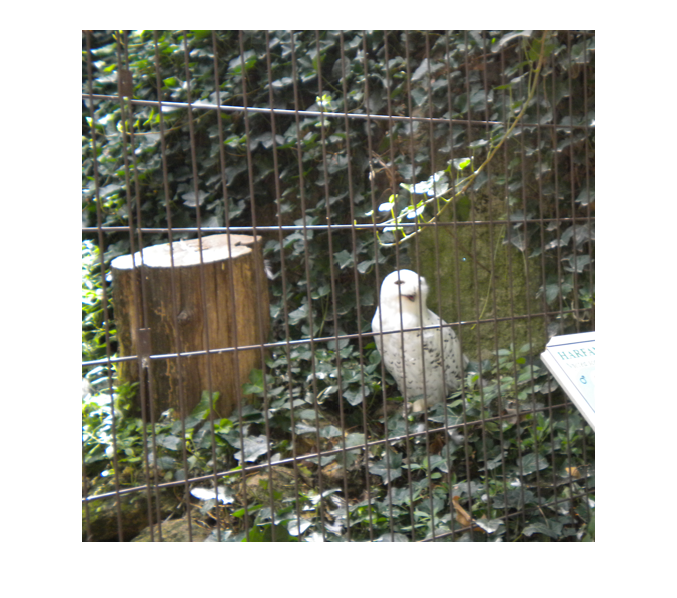
\includegraphics[width = 0.25 \columnwidth]{fig/chouettereduit.png}}
\subfloat[Détection de contours par Canny]{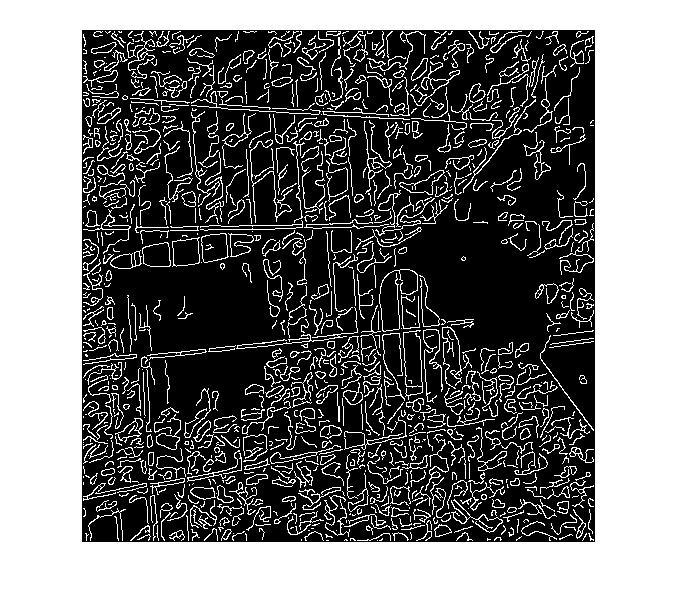
\includegraphics[width = 0.25 \columnwidth]{fig/chouettecanny.png}}
\subfloat[Première détection de lignes]{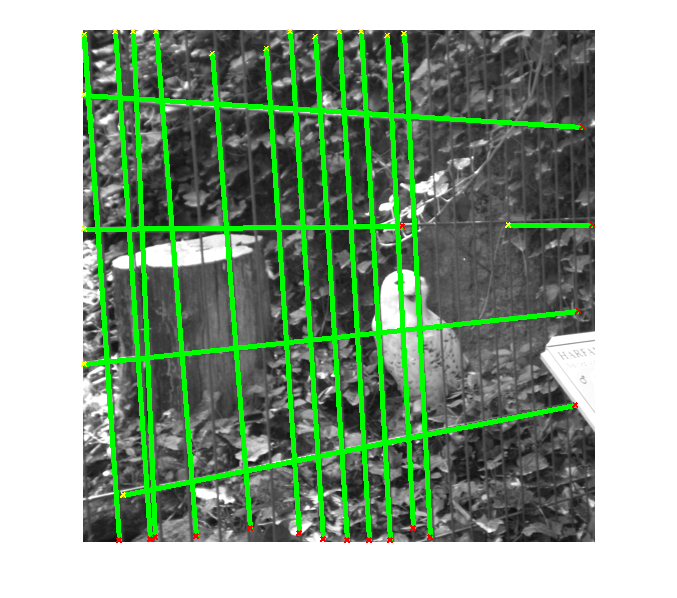
\includegraphics[width = 0.25 \columnwidth]{fig/chouettehough.png}}
\\

\subfloat[Raffinement]{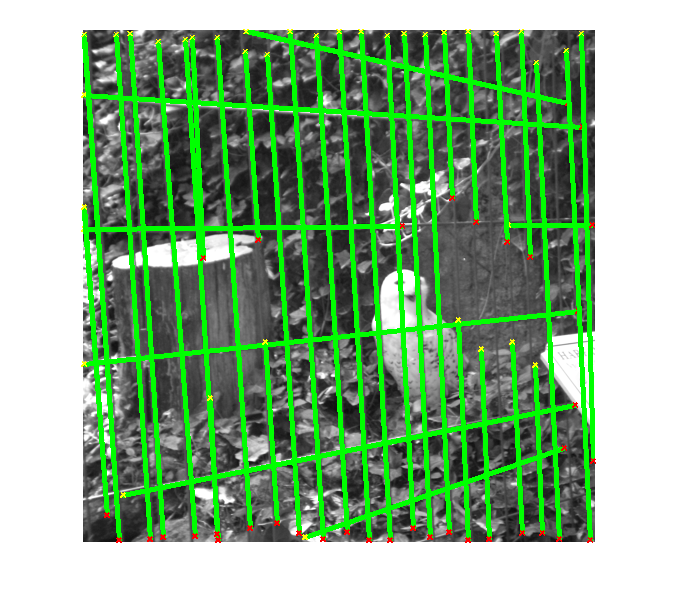
\includegraphics[width = 0.25 \columnwidth]{fig/chouetteraff.png}}
\subfloat[Masque]{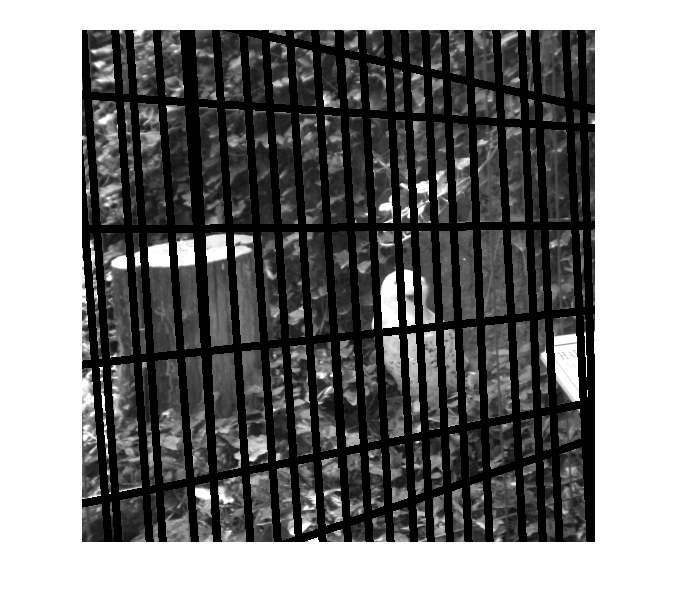
\includegraphics[width = 0.25 \columnwidth]{fig/chouettemask.png}}
\subfloat[Inpainting]{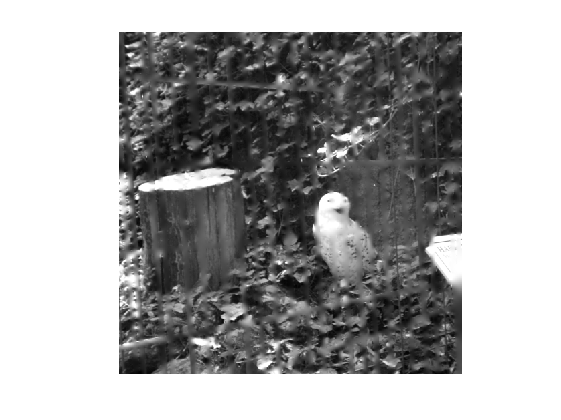
\includegraphics[width = 0.25 \columnwidth]{fig/chouetteinpainting.png}}
\end{tabular}
\caption{\label{résumé}Processus de suppression des lignes d'un grillage sur une image naturelle}
\end{center}
\end{figure}
\end{frame}

\begin{frame}{Exemples de bonnes détections du grillage}
\begin{figure}
\begin{center}
\begin{tabular}{cc}
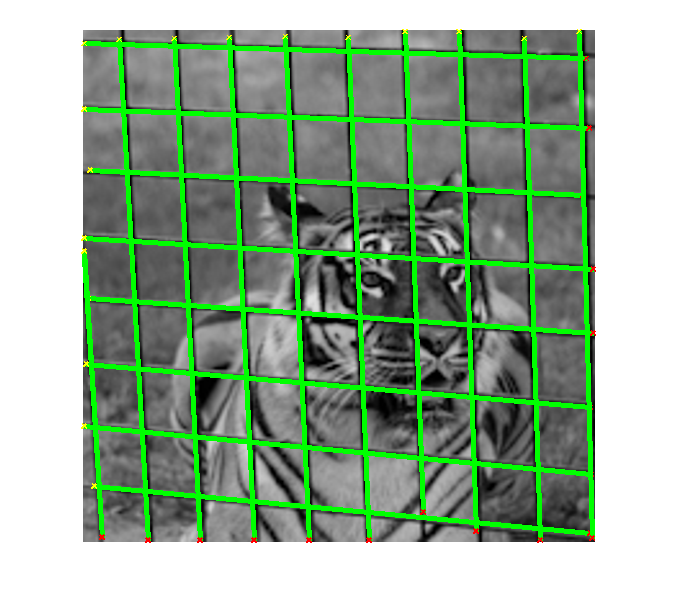
\includegraphics[width = 0.25 \columnwidth]{fig/tigrehough.png}& 
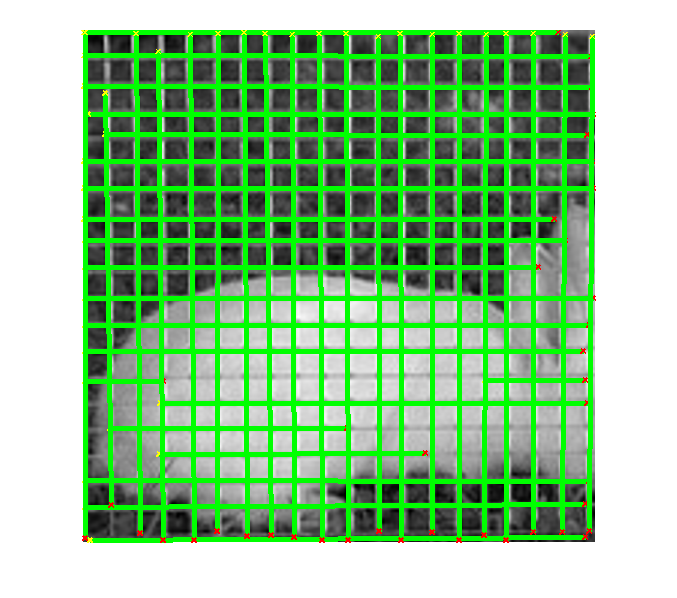
\includegraphics[width = 0.25 \columnwidth]{fig/lapinraff.png}\\
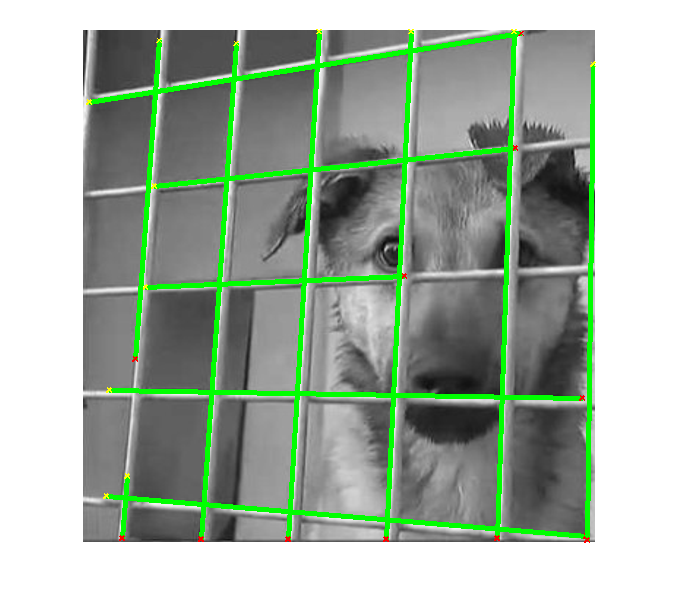
\includegraphics[width = 0.25 \columnwidth]{fig/chiensraff.png}&
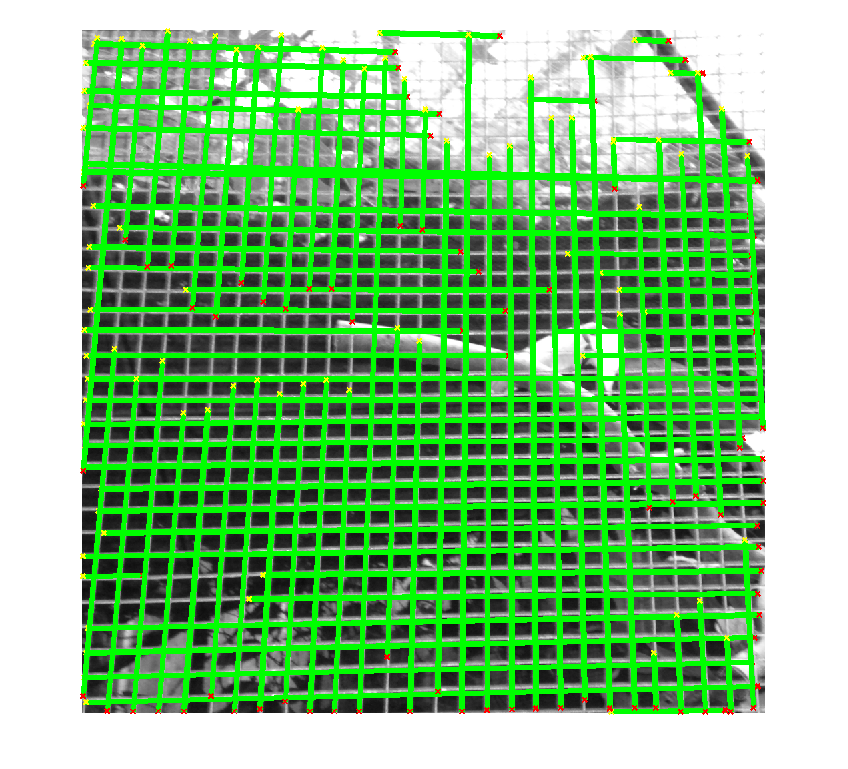
\includegraphics[width = 0.25 \columnwidth]{fig/toucanraff.png}
\end{tabular}
\caption{Exemples de bonnes détections}

\end{center}
\end{figure}

\end{frame}

\begin{frame}{Limites de l'algorithme}
\begin{figure}
\begin{center}
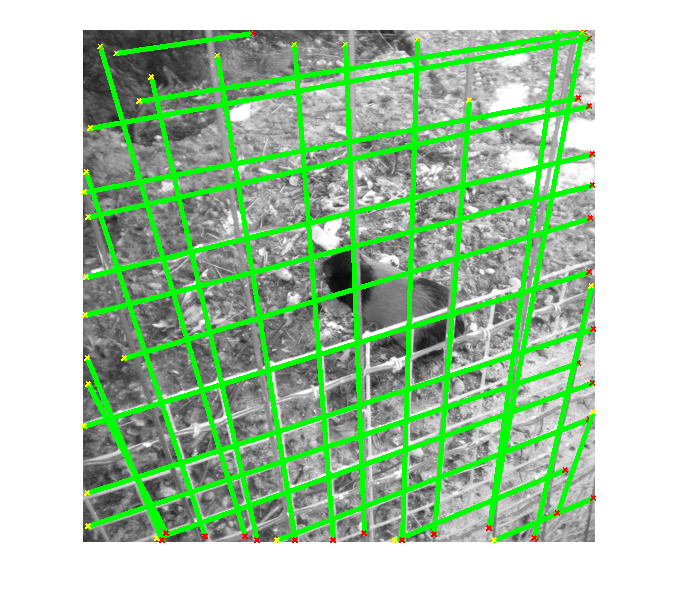
\includegraphics[width = 0.5\columnwidth]{fig/double.png}
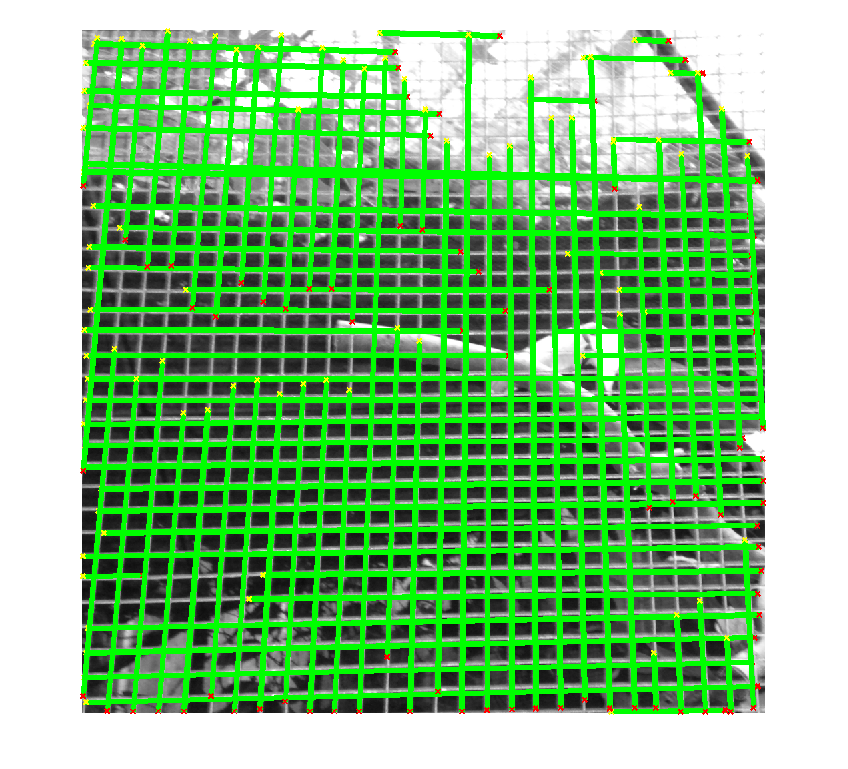
\includegraphics[width = 0.5\columnwidth]{fig/toucanraff.png}
\caption{\label{difficile}Exemples de difficultés pour notre algorithme}
\end{center}
\end{figure}
\end{frame}

\begin{frame}{Limites de notre algorithme}
\begin{figure}
\centering
\begin{tabular}{ccc}
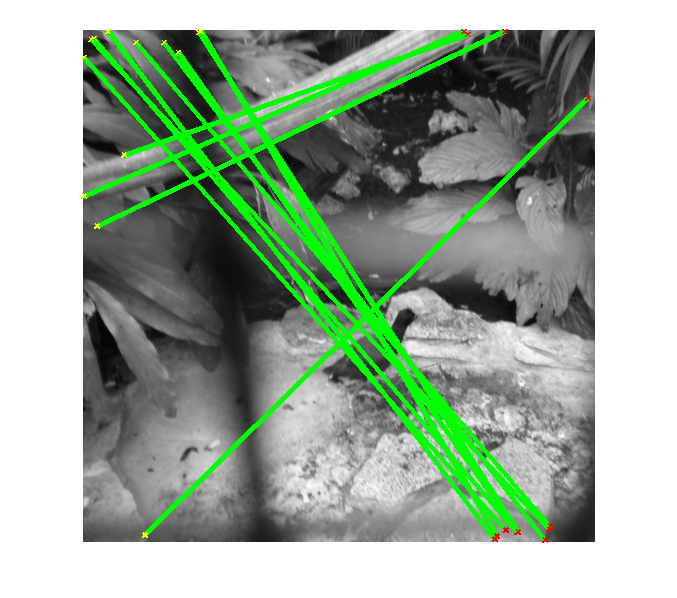
\includegraphics[width = 0.25\columnwidth]{fig/flou.png} &
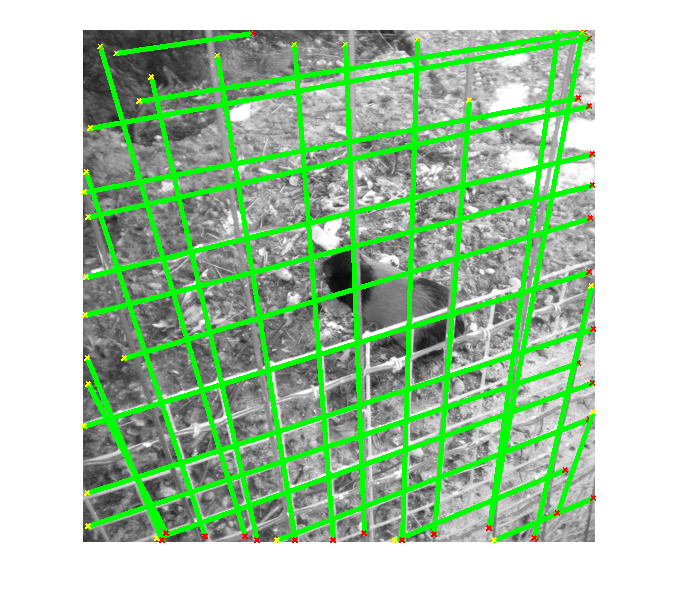
\includegraphics[width = 0.25\columnwidth]{fig/double.png} &
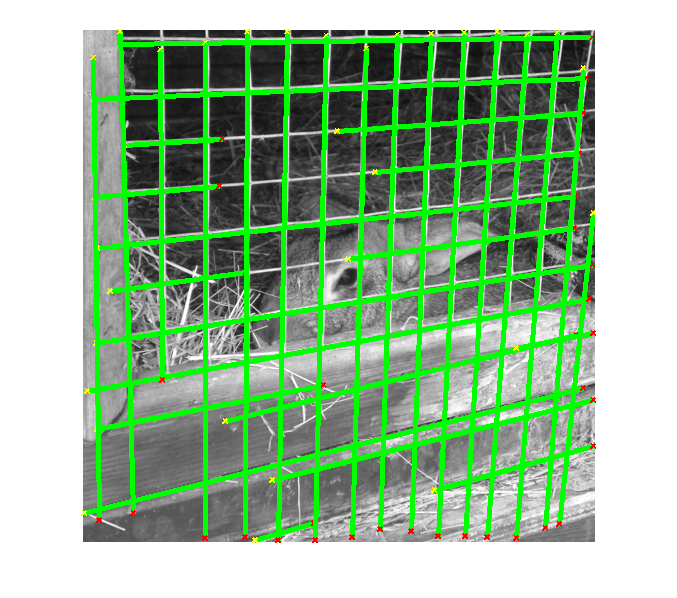
\includegraphics[width = 0.25\columnwidth]{fig/partiel.png}\\
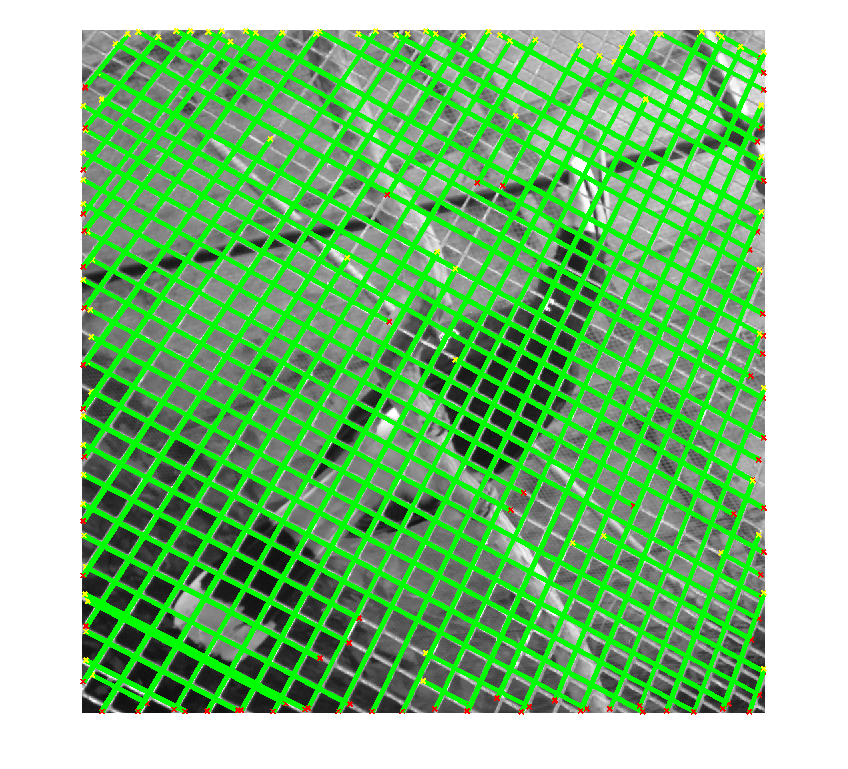
\includegraphics[width = 0.25\columnwidth]{fig/deform.png}&
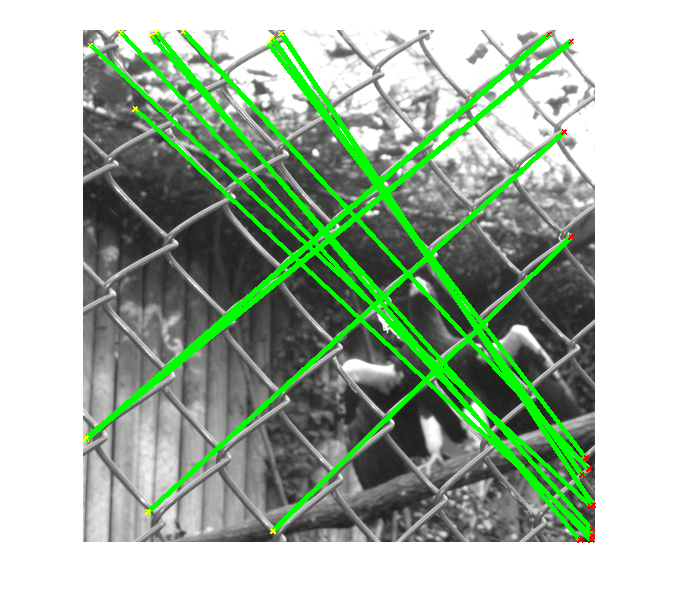
\includegraphics[width = 0.25\columnwidth]{fig/croisillons.png}
\end{tabular}
\caption{\label{badones}Exemples de limites de notre algorithme}
\end{figure}

\end{frame}
